\documentclass[a4paper,12pt]{article} % тип документа

% Поля страниц
\usepackage[left=2.5cm,right=2.5cm,
    top=2cm,bottom=2cm,bindingoffset=0cm]{geometry}
    
%Пакет дял таблиц   
\usepackage{multirow} 
    
%Отступ после заголовка    
\usepackage{indentfirst}


% Рисунки
\usepackage{floatrow,graphicx,calc}
\usepackage{wrapfig}

%%% Работа с картинками
\usepackage{graphicx}  % Для вставки рисунков
\graphicspath{{images/}{images2/}}  % папки с картинками
\setlength\fboxsep{3pt} % Отступ рамки \fbox{} от рисунка
\setlength\fboxrule{1pt} % Толщина линий рамки \fbox{}
\usepackage{wrapfig} % Обтекание рисунков и таблиц текстом

% Создаёем новый разделитель
\DeclareFloatSeparators{mysep}{\hspace{1cm}}

% Ссылки?
\usepackage{hyperref}
\usepackage[rgb]{xcolor}
\hypersetup{				% Гиперссылки
    colorlinks=true,       	% false: ссылки в рамках
	urlcolor=blue          % на URL
}


%  Русский язык
\usepackage[T2A]{fontenc}			% кодировка
\usepackage[utf8]{inputenc}			% кодировка исходного текста
\usepackage[english,russian]{babel}	% локализация и переносы




% Математика
\usepackage{amsmath,amsfonts,amssymb,amsthm,mathtools}

%%% Дополнительная работа с математикой
\usepackage{amsmath,amsfonts,amssymb,amsthm,mathtools} % AMS
\usepackage{icomma} % "Умная" запятая: $0,2$ --- число, $0, 2$ --- перечисление


% Что-то 
\usepackage{wasysym}


\begin{document}
\begin{center}
	\footnotesize{ФЕДЕРАЛЬНОЕ ГОСУДАРСТВЕННОЕ АВТОНОМНОЕ ОБРАЗОВАТЕЛЬНОЕ 			УЧРЕЖДЕНИЕ ВЫСШЕГО ОБРАЗОВАНИЯ}\\
	\footnotesize{МОСКОВСКИЙ ФИЗИКО-ТЕХНИЧЕСКИЙ ИНСТИТУТ\\(НАЦИОНАЛЬНЫЙ 			ИССЛЕДОВАТЕЛЬСКИЙ УНИВЕРСИТЕТ)}\\
	\footnotesize{ФАКУЛЬТЕТ ОБЩЕЙ И ПРИКЛАДНОЙ ФИЗИКИ\\}
	\hfill \break
	\hfill \break
	\hfill \break
	\hfill \break
\end{center}


\begin{figure*}[h]
    \centering
    \includegraphics*[width=10cm,height=7cm,keepaspectratio]{mipt_eng_text_png.png}
    \label{fig:my_label}
\end{figure*}


\begin{center}   
    \hfill \break
	\hfill \break
	\hfill \break
	\hfill \break
	\large{Лабораторная работа № 2.1.6\\\textbf{Эффект Джоуля--Томсона}}\\
	\hfill \break
	\hfill \break
	\hfill \break
	\hfill \break
	\begin{flushright}
		Баранов Даниил\\
		Группа Б02-103
	\end{flushright}
	\hfill \break
	\hfill \break
	\hfill \break
\end{center}
\hfill \break
\hfill \break
\hfill \break
\hfill \break
\begin{center}
	Долгопрудный, 2022 г.
\end{center}
\thispagestyle{empty}



\newpage

\textbf{Цель работы:}
 1) Определение изменения температуры углекислого газа при протекании через малопроницаемую перегородку при разных начальных значениях давления и температуры; 2) вычисление по результатам опытов коэффициентов Ван-дер-Ваальса <<a>> и <<b>>.


\textbf{В работе используются:} трубка с пористой перегородкой; труба Дьюара; термостат; термометры; дифференциальная термопара; микровольтметр; балластный баллон; манометр.
\section{Теоретическая часть}

Эффектом Джоуля–Томсона называется изменение температуры газа, медленно протекающего из области высокого в область низкого давления в условиях хорошей тепловой изоляции. В разреженных газах, которые приближаются по своим свойствам к идеальному газу, при таком течении температура газа не меняется. Эффект Джоуля–Томсона демонстрирует отличие исследуемого газа от идеального.

В работе исследуется изменение температуры углекислого газа при медленном его течении по трубке с пористой перегородкой (риc. \ref{ust}). Трубка 1 хорошо теплоизолирована. Газ из области повышенного давления $ P_1 $ проходит через множество узких и длинных каналов пористой перегородки 2 в область с атмосферным давлением $ P_2 $. Перепад давления $ \Delta P = P_1 - P_2 $ из-за большого сопротивления каналов может быть заметным даже при малой скорости течения газа в трубке. Величина эффекта Джоуля–Томсона определяется по разности температуры газа до и после перегородки.

Рассмотрим стационарный поток газа между произвольными сечениями I и II трубки (до перегородки и после нее). Пусть, для определенности, через трубку прошел 1 моль углекислого газа; $ \mu $ -- его молярная масса. Молярные объемы газа, его давления и отнесенные к молю внутренние энергии газа в сечениях I и II обозначим соответственно $ V_1, P_1, U_1 $ и $ V_2, P_2, U_2 $. Для того чтобы ввести в трубку объем $ V_1 $, над газом нужно совершить работу $ A_1 = P_1V_1 $. Проходя через сечение II, газ сам совершает работу $ A_2 = P_2V_2 $. Так как через боковые стенки не происходит ни обмена теплом, ни передачи механической энергии, то

\begin{equation}\label{1}
A_1-A_2=\left(U_2+\frac{\mu v_2^2}{2}\right) - \left(U_1 + \frac{\mu v_1^2}{2}\right).
\end{equation}

В уравнении \eqref{1} учтено изменение как внутренней (первые члены в скобках), так и кинетической (вторые члены в скобках) энергии газа. Подставляя в \eqref{1} написанные выражения для $ A_1 $ и $ A_2 $ и перегруппировывая члены, найдем

\begin{equation}\label{2}
H_1-H_2=\left(U_1+P_1V_1\right) - \left(U_2 + P_2V_2\right) = \frac{1}{2} \mu \left(v^2_2-v^2_1\right).
\end{equation}

Сделаем несколько замечаний. Прежде всего отметим, что в процессе Джоуля–Томсона газ испытывает в пористой перегородке существенное трение, приводящее к ее нагреву. Потери энергии на нагрев трубки в начале процесса могут быть очень существенными и сильно искажают ход явления. После того как температура трубки установится и газ станет уносить с собой все выделенное им в пробке тепло, формула \eqref{1} становится точной, если, конечно, теплоизоляция трубки достаточно хороша и не происходит утечек тепла наружу через ее стенки.

Второе замечание связано с правой частью уравнения \eqref{2}. Процесс Джоуля–Томсона в чистом виде осуществляется лишь в том случае, если правой частью можно пренебречь, т. е. если макроскопическая скорость газа с обеих сторон трубки достаточно мала. У нас сейчас нет критерия, который позволил бы установить, когда это можно сделать. В силу сохранения энтропии в случае реального газа получаем:

\begin{equation}\label{3}
\mu_\text{Д--Т} = \frac{\Delta T}{\Delta P} \approx \frac{(2a/RT) - b}{C_P}.
\end{equation}

Из формулы \eqref{3} видно, что эффект Джоуля–Томсона для не очень плотного газа зависит от соотношения величин $ a $ и $ b $, которые оказывают противоположное влияние на знак эффекта. Если силы взаимодействия между молекулами велики, так что превалирует <<поправка на давление>>, то основную роль играет член, содержащий $ a $, и 

\[ \frac{\Delta T}{\Delta P} > 0, \]
т. е. газ при расширении охлаждается ($ \Delta T < 0 $, так как всегда $ \Delta P < 0 $). В обратном случае (малые $ a $)

\[ \frac{\Delta T}{\Delta P} < 0, \]
т. е. газ нагревается ($ \Delta T > 0 $, так как по-прежнему $ \Delta P < 0 $).

Этот результат нетрудно понять из энергетических соображений. Как мы уже знаем, у идеального газа эффект Джоуля–Томсона отсутствует. Идеальный газ отличается от реального тем, что в нем можно пренебречь потенциальной энергией взаимодействия молекул. Наличие этой энергии приводит к охлаждению или нагреванию реальных газов при расширении. При больших a велика энергия притяжения молекул. Это означает, что потенциальная энергия молекул при их сближении уменьшается, а при удалении -- при расширении газа -- возрастает. Возрастание потенциальной энергии молекул происходит за счет их кинетической энергии -- температура газа при расширении падает. Аналогичные рассуждения позволяют понять, почему расширяющийся газ нагревается при больших значениях $ b $.

Как следует из формулы \eqref{3}, при температуре \[ T_{\text{инв}} = \frac{2a}{Rb} \] коэффициент $ \mu_\text{Д--Т} $ обращается в нуль. По формулам связи параметров газа Ван-дер-Ваальса с критическими параметрами получаем: 

\begin{equation}\label{4}
T_\text{инв} = \frac{27}{4} T_\text{кр}.
\end{equation}

При температуре $ T_\text{инв} $ эффект Джоуля–Томсона меняет знак: ниже температуры инверсии эффект положителен ($ \mu_\text{Д--Т} > 0 $, газ охлаждается), выше $ T_\text{инв} $ эффект отрицателен ($ \mu_\text{Д--Т} < 0 $, газ нагревается).

Вернемся к влиянию правой части уравнения \eqref{2} на изменение температуры расширяющегося газа. Для этого сравним изменение температуры, происходящее вследствие эффекта Джоуля–Томсона, с изменением температуры, возникающим из-за изменения кинетической энергии газа. Увеличение кинетической энергии газа вызывает заметное и приблизительно одинаковое понижение его температуры как у реальных, так и у идеальных газов. Поэтому при оценках нет смысла пользоваться сложными формулами для газа Ван-дер-Ваальса.

Заменяя в формуле \eqref{2} $ U $ через $ C_VT $ и $ PV $ через $ RT $, найдем

\[ \left(R+C_V\right)\left(T_1-T_2\right)=\mu\left(v_2^2-v_1^2\right)/2 \]
или
\[ \Delta T = \frac{\mu}{2C_P}\left(v_2^2-v_1^2\right). \]

В условиях нашего опыта расход газа $ Q  $ на выходе из пористой перегородки не превышает $ 10 $ см$ ^3 $/с, а диаметр трубки равен 3 мм. Поэтому

\[ v_2<=\frac{4Q}{\pi d^2} = \frac{4\cdot\text{см}^3/\text{с}}{3,14\cdot(0,3)^2\text{ см}^2} \approx 140 \text{ см}/\text{с}. \]

Скорость $ v_1 $ газа у входа в пробку относится к скорости $ v_2 $ у выхода из нее как давление $ P_2 $ относится к $ P_1 $. В нашей установке $ P_1 = 4 $ атм, a $ P_2 = 1 $ атм, поэтому

\[ v_1=\frac{P_2}{P_1}v_2 = 35 \text{ см}/\text{с}. \]

Для углекислого газа $ \mu = 44 $ г/моль, $ C_P = 40 $ Дж/(моль·К); имеем

\[ \Delta T = \frac{\mu}{2C_P}\left(v_2^2-v_1^2\right) \approx 7\cdot10^{-4} \text{ K}. \]

Это изменение температуры ничтожно мало по сравнению с измеряемым эффектом (несколько градусов).

В данной лабораторной работе исследуется коэффициент дифференциального эффекта Джоуля–Томсона для углекислого газа. По экспериментальным результатам оценивается коэффициент теплового расширения, постоянные в уравнении Ван-дер-Ваальса и температура инверсии углекислого газа. Начальная температура газа $ T_1 $ задается термостатом. Измерения проводятся при трех температурах: комнатной, 30 $ ^\circ $C и 50 $ ^\circ $C.

\section{Экспериментальная установка}

\begin{figure}[H]
	\begin{center}
		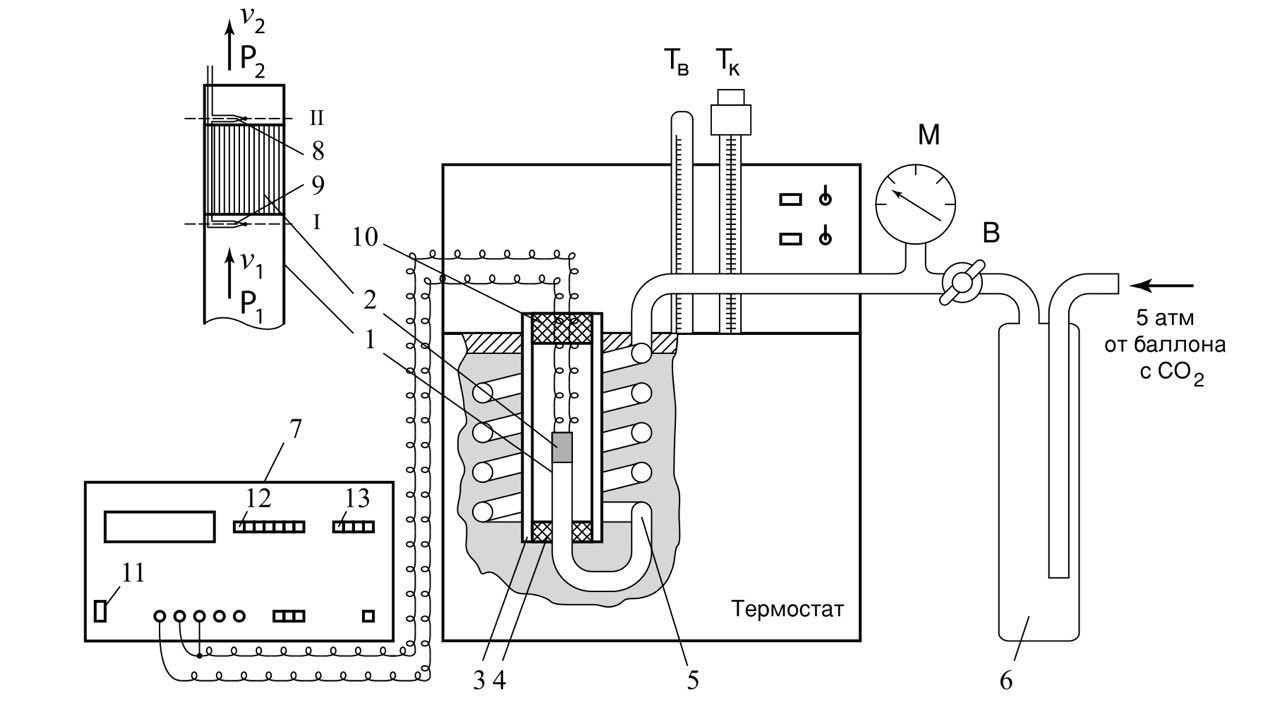
\includegraphics[width=18cm]{2.1.6/ustj.jpg}
	\end{center}
	\caption{Схема установки дял изучения эффектра Джоуля--Томсона}
	\label{ust}
\end{figure}

Схема установки для исследования эффекта Джоуля–Томсона в углекислом газе представлена на рисунке \ref{ust}. Основным элементом установки является трубка 1 с пористой перегородкой 2, через которую пропускается исследуемый газ. Трубка имеет длину 80 мм и сделана из нержавеющей стали, обладающей, как известно, малой теплопроводностью. Диаметр трубки $ d = 3 $~мм, толщина стенок 0,2 мм. Пористая перегородка расположена в конце трубки и представляет собой стеклянную пористую пробку со множеством узких и длинных каналов. Пористость и толщина пробки ($ l = 5 $ мм) подобраны так, чтобы обеспечить оптимальный поток газа при перепаде давлений $ \Delta P = 4 $ атм (расход газа составляет около $ 10 $ см$ ^3 $/с); при этом в результате эффекта Джоуля–Томсона создается достаточная разность температур.

Углекислый газ под повышенным давлением поступает в трубку через змеевик 5 из балластного баллона 6. Медный змеевик омывается водой и нагревает медленно протекающий через него газ до температуры воды в термостате. Температура воды измеряется термометром $ T_\text{в} $, помещенным в термостате. Требуемая температура воды устанавливается и поддерживается во время эксперимента при помощи контактного термометра $ T_\text{к} $.

Давление газа в трубке измеряется манометром М и регулируется вентилем В (при открывании вентиля В, т. е. при повороте ручки против часовой стрелки, давление $ P_1 $ повышается). Манометр М измеряет разность между давлением внутри трубки и наружным (атмосферным) давлением. Так как углекислый газ после пористой перегородки выходит в область с атмосферным давлением $ P_2 $, то этот манометр непосредственно измеряет перепад давления на входе и на выходе трубки $ \Delta P = P_1 - P_2 $.

Разность температур газа до перегородки и после нее измеряется дифференциальной термопарой медь -- константан. Константановая проволока диаметром 0,1 мм соединяет спаи 8 и 9, а медные проволоки (того же диаметра) подсоединены к цифровому вольтметру 7. Отвод тепла через проволоку столь малого сечения пренебрежимо мал. Для уменьшения теплоотвода трубка с пористой перегородкой помещена в трубу Дьюара 3, стенки которой посеребрены, для уменьшения теплоотдачи, связанной с излучением. Для уменьшения теплоотдачи за счет конвекции один конец трубы Дьюара уплотнен кольцом 4, а другой закрыт пробкой 10 из пенопласта. Такая пробка практически не создает перепада давлений между внутренней полостью трубы и атмосферой.

\section{Результаты измерений}

Во время проведения эксперимента температура и давление в комнате были соответственно равны $T_\text{к} = 23,4 ^\circ C$ и $p_0 = 100,1 $кПа.

\floatsetup[table]{capposition=top}
\begin{table}[H]
    \begin{tabular}{|c|c||c|c|}
    \hline
    \multicolumn{2}{|c||}{$T = 17 ^\circ C$} & \multicolumn{2}{|c|}{$T = 25,2 ^\circ C$} \\ \hline
    $\Delta p$, бар & $\Delta U$, мкВ & $\Delta p$, бар & $\Delta U$, мкВ \\ \hline
    4,05 & 148 & 4,05 & 150 \\ \hline
    3,75 & 130 & 3,8  & 128 \\ \hline
    3,5  & 120 & 3,35 & 110 \\ \hline
    3,0  & 100 & 2,85 & 89 \\ \hline
    2,55 & 80  & 2,15 & 64 \\ \hline \hline
    \multicolumn{2}{|c||}{$T = 35 ^\circ C$} & \multicolumn{2}{|c|}{$T = 50 ^\circ C$} \\ \hline 
    $\Delta p$, бар & $\Delta U$, мкВ & $\Delta p$, бар & $\Delta U$, мкВ \\ \hline
    4   & 135 & 4,1 & 127 \\ \hline
    3,3 & 98  & 3,5 & 97 \\ \hline
    2,9 & 80  & 2,9 & 74 \\ \hline
    2,4 & 60  & 2,3 & 53 \\ \hline
    \label{results}
    \end{tabular}
    \caption {Результаты показаний вольтметра в зависимости от разности давления}
\end{table}

Погрешности показаний приборов составили 
    $\sigma_p=0,1$ бар и 
    $\sigma_U=2$ мкВ.
    
Также для последующей обработки данных необходимо будет учитывать зависимость от температуры чувствительности термопары медь--константан.

\begin{table}[H]
    \begin{tabular}{|c|c|c|c|c|c|}
    \hline
    Температура, $^\circ C$ & 0-10 & 10-20 & 20-30 & 30-40 & 40-50 \\ \hline
    мкВ$/^\circ C$ & 38,9 & 39,8 & 40,7 & 41,6 & 42,5 \\ \hline
    \end{tabular}
    \label{sensitivity}
    \caption {Зависимости приведённого напряжения от температуры}
\end{table}

\section{Обработка результатов измерений}

По данным в таблицах 1 и 2 построим график зависимости $\Delta T(\Delta p)$ (\ref{DTDP}).

\begin{figure}[H]
    \centering
    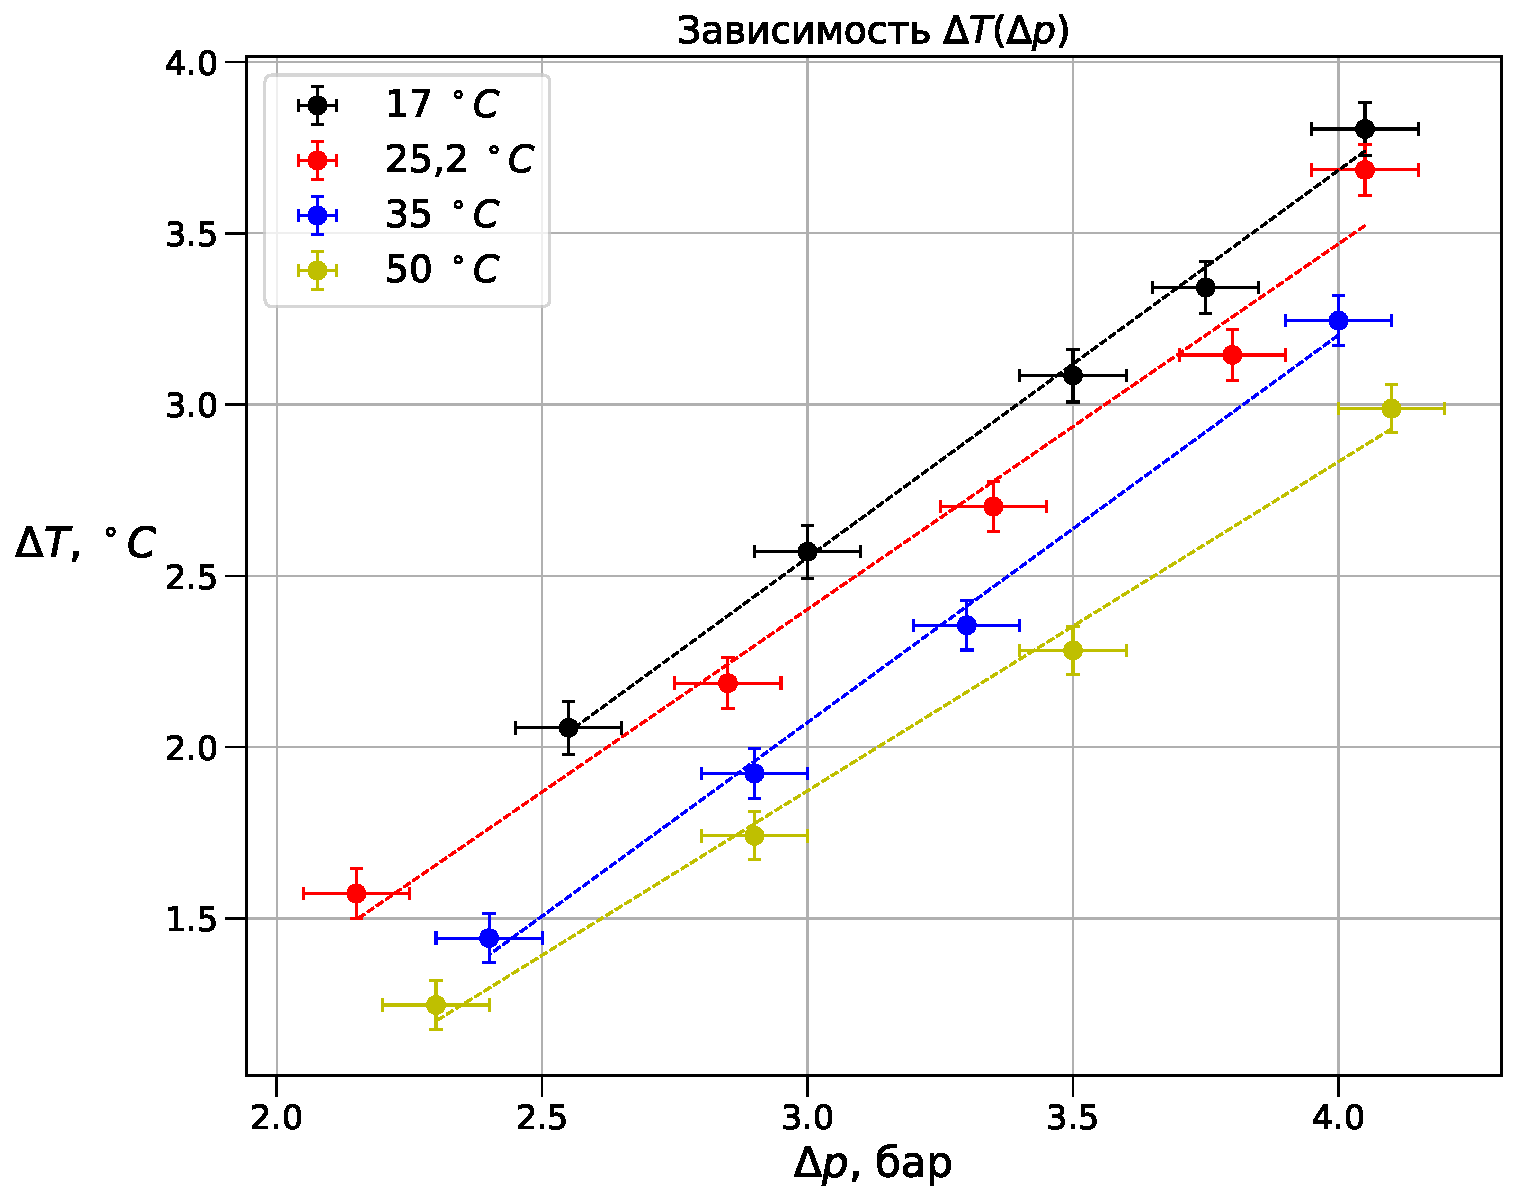
\includegraphics[scale=0.65]{2.1.6/DPDT.pdf}
    \caption{Зависимость $\Delta T(\Delta p)$}
    \label{DTDP}
\end{figure}

Из наклона графиков найдем соответствующие коэффициенты:

\begin{center}
    $\displaystyle \mu_{17} = 1.13 \pm 0.04\  K/$бар, $\displaystyle \sigma_{\mu} = 3\%$;\break
    $\displaystyle \mu_{25} = 1.07 \pm 0.07\  K/$бар, $\displaystyle \sigma_{\mu} = 7\%$;\break
    $\displaystyle \mu_{35} = 1.13 \pm 0.04\  K/$бар, $\displaystyle \sigma_{\mu} = 3\%$;\break
    $\displaystyle \mu_{50} = 0.96 \pm 0.04\  K/$бар, $\displaystyle \sigma_{\mu} = 4\%$.\break
\end{center}

Вычислим параметры газа Ван-дер-Ваальса, используя коэффициенты $ \mu_\text{Д--Т} $, полученные для разных пар температур.

Пользуясь формулой \eqref{3}, получим:
\begin{center}
    $\displaystyle a = \frac{\left(\mu_1 - \mu_2\right)C_PRT_1T_2}{2\left(T_2-T_1\right)}$,\break\break
	$\displaystyle b = \frac{C_P(\mu_2T_2-\mu_1T_1)}{T_1-T_2}. $

\end{center}

После вычислений были получены следующие величины:

\begin{center}
    $\displaystyle a_{17-25}= 0.78 \pm 0.09 \  \frac{\text{Па}\cdot \text{м}^6}{\text{моль}^2}$, $\displaystyle \sigma_{a} = 11,5 \%$; \break
    
    $\displaystyle a_{35-50}= 1.36 \pm 0.16 \  \frac{\text{Па}\cdot \text{м}^6}{\text{моль}^2}$, $\displaystyle \sigma_{a} = 11,5 \%$; \break

    $\displaystyle b_{17-25}= 9.18 \pm 0.92 \cdot 10^{-5} \ \frac{\text{м}^3}{\text{моль}}$, $\displaystyle \sigma_{b} = 10 \%$; \break
    
    $\displaystyle b_{35-50}= 21.0 \pm 2.0 \cdot 10^{-5} \ \frac{\text{м}^3}{\text{моль}}$, $\displaystyle \sigma_{b} = 10 \%$. \break
\end{center}

Сверим полученные результаты с табличными. Согласно справочнику для углекислого газа
\begin{center}
    
$\displaystyle a = 0,36 \  \frac{\text{Па}\cdot\text{м}^6}{\text{моль}^2}$; \break$\displaystyle b = 4,2\cdot 10^{-5} \ \frac{\text{м}^3}{\text{моль}}.$ 
\end{center}
Полученные данные значительно отличаются от табличных.

Используя формулу \eqref{4}, по полученным параметрам газа Ван-дер-Ваальса вычислим $ T_\text{инв} $. Также оценим погрешность по следующей формуле:
$\displaystyle \sigma_{T_\text{инв}} = T_\text{инв}\sqrt{\varepsilon^2_a+\varepsilon_b^2}.$

\begin{center}
    $\displaystyle T_{17-25} = 2045 K$, $\displaystyle \sigma_{T_{\text{инв}}} = 15\%$; \break
    
    $\displaystyle T_{35-50} = 1559 K$, $\displaystyle \sigma_{T_{\text{инв}}} = 15\%$.
\end{center}

Для углекислого газа, согласно справочнику  \[ T_\text{инв} = 2053 \text{ K}.\]

На этот раз полученные результаты не так сильно отличаются от табличных. Сильное отличие результатов от табличных данным говорит о несостоятелности формулы Ван-дер-Ваальса как количественного приближения, оставаясь при этом общепринятой качественной моделью описания реальных газов.

\end{document}
